

   
\documentclass[journal,12pt,twocolumn]{beamer}
\usetheme{CambridgeUS}

\usepackage[utf8]{inputenc}
\usepackage{tfrupee}
\usepackage{enumitem}
\usepackage{amsmath}
\usepackage{amssymb}
\usepackage{graphicx}
\usepackage{mathtools}
\providecommand{\sbrak}[1]{\ensuremath{{}\left[#1\right]}}
\providecommand{\lsbrak}[1]{\ensuremath{{}\left[#1\right.}}
\providecommand{\rsbrak}[1]{\ensuremath{{}\left.#1\right]}}
\providecommand{\brak}[1]{\ensuremath{\left(#1\right)}}
\providecommand{\lbrak}[1]{\ensuremath{\left(#1\right.}}
\providecommand{\rbrak}[1]{\ensuremath{\left.#1\right)}}
\providecommand{\cbrak}[1]{\ensuremath{\left\{#1\right\}}}
\providecommand{\lcbrak}[1]{\ensuremath{\left\{#1\right.}}
\providecommand{\rcbrak}[1]{\ensuremath{\left.#1\right\}}}
\newcommand{\myvec}[1]{\ensuremath{\begin{pmatrix}#1\end{pmatrix}}}
\let\vec\mathbf

\title{Assignment 9}
\author{Sai Pradeep AI21BTECH11013}
\date {\today}

\begin{document}
\begin{frame}
 \maketitle   
\end{frame}

\begin{frame}{Contents}
    \tableofcontents
\end{frame}

\section{Question}
\begin{frame}{Question : Ex. 8.11 , Papoulis}
\begin{block}

Q: In an exit poll of 900 voters questioned, 360 responded that they favor a particular proposition. On the basis, it was reported that 40\% of the voters favor the proposition.(a) Find the margin of error if the confidence coefficient of the results is 0.95.(b) Find the confidence coefficient if the margin of error is $\pm 2 \%$.
\end{block}
\end{frame}
\section{Solution}
\begin{frame}{Solution}
\begin{enumerate}[label=(\alph*)]
\item    For this problem, 
We know that $\bar{x}=0.40$, $n=900 and z_u \approx 2:$\\
Hence, Margin of error:
\begin{align}
\label{eq:1}
 \pm 100 z_u \sqrt \frac{\bar{x}\brak{1-\bar{x}}}{n}&= \pm 3.27\%
\end{align}
\item We wish to find $z_u$.
\end{enumerate}
\begin{align}
 \pm 100 z_{u} \sqrt \frac{\bar{x}\brak{1-\bar{x}}}{n}&=2
 z_{u}&=1.225
\end{align}
Hence $u=0.89$\\
This yields the confidence coefficient,
\begin{align}
 \gamma=2 \times u \\
Hence, \gamma=0.78
\end{align}
\end{frame}
\begin{frame}{Python Output}
\section{Code output}
   \begin{figure}[htb!]
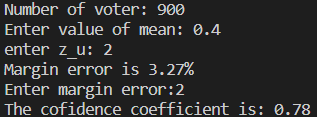
\includegraphics[width=10cm]{figures/python_output.png}
\caption{python code output}
\end{figure}
\end{frame}
\end{document}
